\chapter{Grundlagen}
\label{chap:hess-smith}


\section{Hess-Smith-Panelverfahren}
\begin{figure}[!h]
\begin{center} 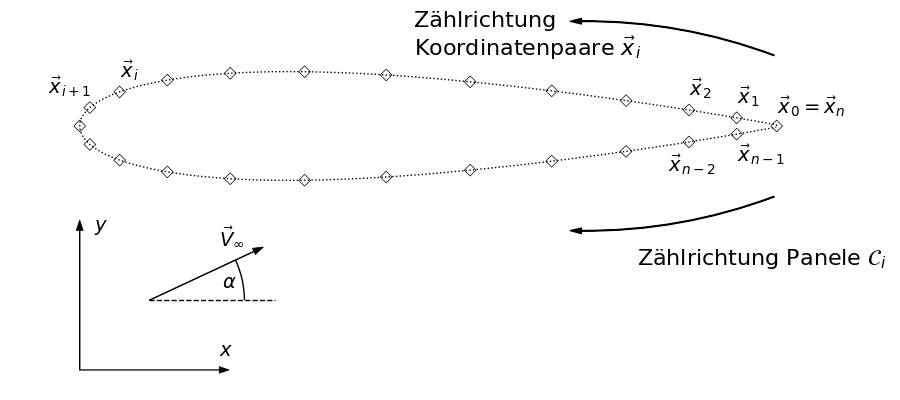
\includegraphics[scale=0.3]{figures/zaehlrichtung.png} \end{center}
\caption{Zur Definition der Zählrichtung der Panels sowie der Anströmgeschwindigkeit und deren Winkel}
\label{fig:zaehlrichtung}
\end{figure}
Das Hess-Smith-Panelverfahren ist ein Verfahren zur Berechnung von ebenen Potentialströmungen um geschlossene Körper mit Auftrieb. Ein kontinuierlicher zweidimensionaler Körper mit der Umfangkurve $\mathcal{C}$ wird dabei zunächst durch  $n + 1$ diskrete Datenpunkte $\vec x_i = (x_i, y_i)$ dargestellt. Die Zählrichtung dieser Punkte sei als im Uhrzeigersinn festgelegt (siehe Abb. \ref{fig:zaehlrichtung}). Für das Profil gilt somit die Periodizität $\vec x_n = \vec x_0$.\\
Die Kontur des Profils wird nun durch eine endliche Anzahl Verbindungsgeraden zwischen zwei benachbarten Punkten $\vec x_i, \vec x_{i+1}$, den Panelen $\mathcal{C}_i$ (Abb. \ref{fig:panel}) angenähert. Dabei wird jedes Panel durch die folgenden Parameter charakterisiert:
\begin{itemize}
\item Den Mittelpunkten auf beiden Achsen: 
\begin{equation}
X_i =  \frac{x_{n-i}+x_{n-i-1}}{2}, \; Y_i =  \frac{y_{n-i}+y_{n-i-1}}{2},
\end{equation}
\item seinem Neigungswinkel: 
\begin{equation}
\theta_i =  \left( \frac{y_{n-i-1} - y_{n-i}}{x_{n-i-1} - x_{n-i}} \right),
\end{equation}
\item und seiner Länge: 
\begin{equation}
l_i =  \sqrt{(x_{n-i-1} - x_{n-i})^2 + (y_{n-i-1} - y_{n-i})^2}.
\end{equation}
\end{itemize}


\begin{figure}
\begin{center} 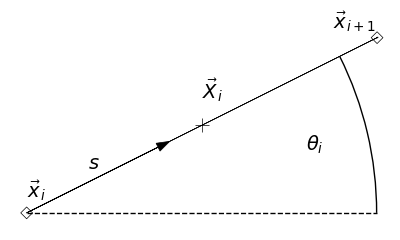
\includegraphics[scale=0.5]{figures/panel.png} \end{center}
\caption{Zur Definition eines Panels}
\label{fig:panel}
\end{figure}

Im Hess-Smith-Panelverfahren sei nun jedes dieser Panels mit einer vorerst unbestimmten, konstanten Quelldichte $q_i$ behaftet, welche an einem Punkt $\vec r_i =  \vec x - \hat x_i(s)$ zum Geschwindigkeitspotential den Beitrag
\begin{equation}
\label{eqn:potq}
\phi_i^{(q)} =  \frac{q_i}{2 \pi } \int_{\mathcal{C_i}} ds \ln r_i
\end{equation}
liefert. $s$ ist dabei die Koordinate der Bogenlänge, welche das gesamte Profil parametrisiert. \\
Ebenso liefert die Profilanströmung mit der konstanten Geschwindigkeit $V_{\infty}$ unter dem Winkel $\alpha $ ein Potential
\begin{equation}
\label{eqn:potv}
\phi_{\infty} =  V_{\infty} (\cos \alpha x + \sin \alpha y).
\end{equation}
Aus der Summe über alle Panelbeiträge aus (\ref{eqn:potq}) und (\ref{eqn:potv}) ergibt sich das Gesamtgeschwindigkeitspotential zu
\begin{equation}
\label{eqn:potnovortex}
\phi(\vec x) =  V_{\infty} (\cos \alpha x + \sin \alpha y) + \sum_{i=0}^{n-1} \phi_i^{(q)}.
\end{equation}
Daraus folgt für die Geschwindigkeit im Punkte $\vec x$ 
\begin{equation}
\vec v ( \vec x) =  \nabla  \phi (\vec x).
\end{equation}
Auf der Oberfläche des Profils muss die Strömung die Gleitbedingung erfüllen; damit lassen sich $n$ Gleichungen aufstellen, um diese Bedingung zu modellieren. Wir verlangen, dass die Normalkomponente des Geschwindigkeitsvektors,
\begin{equation}
v_j^{(n)} =  \vec v(\vec X_j) \cdot \vec n_j,
\end{equation}
verschwindet. Dabei ist $\vec n_j$ der Normalvektor auf das Panel $\mathcal{C}_j$.\\
Wir erhalten in 0. Ordnung ein System von $n$ Gleichungen
\begin{equation}
\label{eq:lgls1}
\sum_{j=0}^{n-1} M_{ij}^{(q)}q_j =  b_i,
\end{equation}
mit
\begin{equation}
M_{ij}^{(q)} = \frac{1}{q_j} \nabla \phi_j^{(q)} (\vec X) \cdot \vec n_i,
\end{equation}
\begin{equation}
b_i =  -V_{\infty} \left( \begin{matrix} \cos \alpha \\ \sin \alpha \end{matrix} \right) \cdot \vec n_i,
\end{equation}
aus dessen Lösung wir die Quellstärken $q_i$ für jedes Panel ermitteln können. \\
Damit kann nun der Tangentialkomponenten des Geschwindigkeitsvektors
\begin{equation}
\label{eqn:vt}
v_j^{(t)} =  \vec v(X_j) \cdot \frac{\vec x_{j+1}-\vec x_j}{|\vec x_{j+1}-\vec x_j|},
\end{equation}
bestimmt werden. \\
Aus der Bernoulli-Gleichung
\begin{equation}
p_{\infty} + \frac{1}{2} \rho V_{\infty}^2 =  p + \frac{1}{2} \rho v^2,
\end{equation}
definieren wir den Druckbeiwert als das Verhältnis zwischen der Druckdifferenze zwischen der Profilanströmung und dem dynamischen Druck 
\begin{equation}
c_p =  \frac{p-p_{\infty}}{\frac{1}{2} \rho V_{\infty}^2}.
\end{equation}
Daraus können wir den Druckbeiwert
\begin{equation}
c_{p_j} =  1 - \left( \frac{v_j^{(t)}}{V_{\infty},}\right)
\end{equation}
am Mittelpunkt des Panels $\mathcal{C}_j$ bestimmen.
\subsection{Berücksichtigung einer Wirbelbewegung}
Wollen wir den Auftrieb berücksichtigen, so reicht die reine Quellbelegung des Profils noch nicht aus. \\
Im Hess-Smith Verfahren nehmen wir für das gesamte Profil eine einzige konstante Wirbelbelegung $\gamma$ für alle Panels an. Damit wird das Potential (\ref{eqn:potnovortex}) erweitert um Beiträge
\begin{equation}
\phi_i^{(w)} =  \frac{\gamma}{2 \pi } \int ds \theta_i,
\end{equation}
zu
\begin{align}
\phi(\vec x) &=  V_{\infty} (\cos \alpha x + \sin \alpha y) + \sum_{i=0}^{n-1} \left( \phi_i^{(q)} + \phi_i^{(w)} \right) \nonumber \\
&= V_{\infty} (\cos \alpha x + \sin \alpha y) + \sum_{i=0}^{n-1} \int_{\mathcal{C}_i} \left( \frac{q_i}{2\pi } \ln r_i - \frac{\gamma}{2\pi } \theta_{i} \right) ds ´´
\end{align}
Die Gleitbedingung bleibt erhalten, allerdings muss das Gleichungssystem aber entsprechend dem hinzugekommenen Geschwindigkeitsbeitrag erweitert werden. Für die neue Unbekannte $\gamma$ fehlt also eine Gleichung. Diese ergibt sich aus der Kutta-Bedingung, welche besagt, dass es an der Hinterkante des Profils keine Umströmung gibt.\\
Zur Modellierung der Kutta-Bedingung wählen wir
\begin{equation}
v_0^{(t)} =  -v_n^{(t)}.
\end{equation} 
Daraus folgt, dass die Tangentialkomponenten des Geschwindigkeitsvektors in den Mittelpunkten der Panels, welche die Profilhinterkante bilden, vom Betrag gleich groß und gegenläufig gerichtet sein muss (siehe Abb. \ref{fig:kutta}). \\
Nach Lösung des erhaltenen linearen Gleichungssystems mit $q_n = \gamma$ können wir nun den Auftriebsbeiwert $c_a$ ermitteln. Dieser ergibt sich mit $t$, der Proftiltiefe und $l_i$, der Länge des Panels $\mathcal{C}_i$, approximiert in folgender Form:
\begin{equation}
c_a \approx \frac{2}{V_{\infty t}}\sum_{i=0}^{n-1} v_i^{(t)} l_i.
\end{equation}
\begin{figure}
\begin{center} 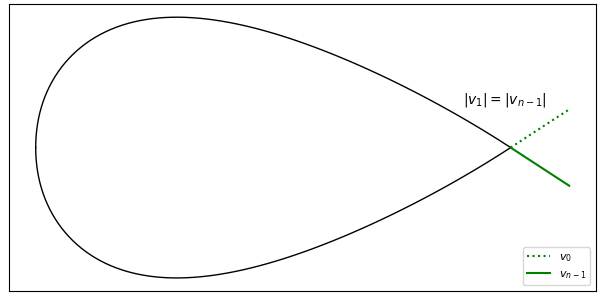
\includegraphics[scale=0.7]{figures/kutta.png} \end{center}
\caption{Zur Kutta-Bedingung am Beispiel eines NACA0012-Profils - am Punkt der Hinterkante sind die Tangentialgeschwindigkeiten genau entgegengerichtet}
\label{fig:kutta}
\end{figure}
Für eine analytische Berechnung des Auftriebsbeiwerts müssen wir nun noch die Systemmatrix bestimmen, welche das lineare Gleichungssystem (\eqref{eq:lgls1}) definiert. \cite{Hess:1966} \cite{Cebeci:1999} \cite{Alonso:2005}

\subsection{Berechnung der Systemmatrix}
\label{chap:systemmatrixtheory}
Die Systemmatrix zur Berechnung der Normalgeschwindigkeiten $v_i^{(n)}$ in den Panelmittelpunkten für eine stückweise konstante Quellenbewegung der Panels ergibt sich aus der Gleitbedingung. Wenden wir diese direkt auf \ref{eqn:potnovortex} an, muss ein kompliziertes Integral gelöst werden. Dieses kann theoretisch direkt mit Computermethoden gelöst werden, für den Berechnungsaufwand ist es allerdings gerade bei Profilen mit einer hohen Anzahl an Panels günstiger, dieses analytisch zu berechnen. \\
Für die Systemmatrix und ihre Parameter gelten:
\begin{equation}
M_{ij} = A_{ij}^{(n)}, \;\; i = 0, 1, \ldots , n-1; \;\; j = 0,1,\ldots , n-1.
\end{equation}
mit der Einflussmatrix der Quellbelegung
\begin{equation}
A_{ij}^{(n)} = -\sin {(\theta _i - \theta _j)} I_{ij} + \cos{(\theta _i - \theta _j)} J_{ij}
\end{equation}
sowie das geometrische Integral der Normalgeschwindigkeit
\begin{equation}
I_{ij} = 
     \begin{cases}
       \frac{1}{4\pi } \ln \left[ \frac{(l_j + 2 \xi_{ij})^2 + 4 \eta_{ij}^2}{(l_j -2 \xi _{ij})^2 + 4 \eta_{ij}^2} \right] &\quad i \neq j \\
       0 &\quad i = j \\
     \end{cases}
\end{equation}
und dem geometrischen Integral der Tangentialgeschindigkeit
\begin{equation}
J_{ij} = 
     \begin{cases}
       \frac{1}{2\pi } \arctan \left[ \frac{l_j - 2 \xi_{ij}}{2 \eta_{ij}} \right] + \frac{1}{2\pi } \arctan \left[ \frac{l_j + 2 \xi_{ij}}{2 \eta_{ij}} \right] &\quad i \neq j \\
       \frac{1}{2} &\quad i = j \\
     \end{cases}
\end{equation}
\begin{equation}
\xi_{ij} =  (X_i - X_j) \cos \theta _j + (Y_i - Y_j) \sin \theta _j
\end{equation}
\begin{equation}
\eta_{ij} =  -(X_i - X_j) \sin \theta _j + (Y_i - Y_j) \cos \theta _j
\end{equation}
Mit der Systemmatrix und den Inhomogenitäten $b_i$ können wir nun das lineare Gleichungssystem aus (\ref{eq:lgls1}) berechnen. \\
Für die Tangentialkomponente der Geschwindigkeit erhalten wir dann den Ausdruck
\begin{equation}
\label{eq:vtnovortex}
v_i^{(t)} =  \sum_{j=0}^{n-1} A_{ij}^{(t)} q_j + V_{\infty} \cos{(\alpha - \theta_i)},
\end{equation}
mit der Einflussmatrix der Wirbelbelegung
\begin{equation}
A_{ij}^{(t)} =  \cos{(\theta _i - \theta _j)} I_{ij} + \sin{(\theta _i - \theta _j)} J_{ij}.
\end{equation}
\\
Diese Systemmatrix berücksichtigt allerdings noch keine Wirbelbelegungen. Im Falle einer konstanten Wirbelbelegung $\gamma$ auf allen Panels erweitert sich die Dimension von $M_{ij}$ von $n \times n$ auf $(n+1) \times (n+1)$. Dadurch müssen folgende zusätzliche Elemente bestimmt werden:
\begin{equation}
M_{in} =  \sum_{j=0}^{n-1} A_{ij}^{(t)}, \;\; i=0,1,\ldots, n-1;
\end{equation}
\begin{equation}
M_{nj} =  A_{0j}^{(t)} + A_{n-1,j}^{(t)}, \;\; j =0,1,\ldots, n-1;
\end{equation}
\begin{equation}
M_{n,n} =  - \sum_{j=0}^{n-1} \left[ A_{0,j}^{(n)} + A_{n-1,j}^{(n)}\right];
\end{equation}
\begin{equation}
b_n =  -V_{\infty} [\cos{(\alpha -\theta 0)} + \cos{(\alpha -\theta _{n-1})}];
\end{equation}
Gleichung (\ref{eq:vtnovortex}) erweitert sich damit zu
\begin{equation}
v_i^{(t)} =  \sum_{j=0}^{n-1} A_{ij}^{(t)} q_j - \gamma \sum_{j=0}^{n-1}A_{i,j}^{(n)} + V_{\infty} \cos{(\alpha - \theta_i)}.
\end{equation}
\newpage
\chapter{Bericht der Arbeit}
Im Folgenden werden die wesentlichen Erkenntnisse der Arbeit präsentiert.
\section{Vorbereitung der Daten}
Die Daten der Profile wurden der UIUC Airfoil Data Site\footnote{\url{https://m-selig.ae.illinois.edu/ads/coord_database.html}} entnommen. Die Daten lagen dabei überwiegend im Selig- oder Lednicer-Format vor.\footnote{Eine Gegenüberstellung der beiden Formate ist in \nameref{appendix:a} zu finden.}
\\
Im Lednicer-Format wird in der ersten Zeile die Bezeichnung des Profils angegeben. In der zweiten Zeile wird die Anzahl der Koordinatenpaare der Ober- und Unterseite angegeben. Ab der dritten Zeile werden die Koordinaten der Panelenden $(x_i,y_i)$ von $x=0$ bis $x=1$ für die Oberseite des Profils angegeben. Danach folgt eine Leerzeile. Danach werden die Koordinaten der Panelenden $(x_i,y_i)$ von $x=0$ bis $x=1$ für die Unterseite des Profils angegeben.
\\
Im Selig-Format wird in der ersten Zeile die Bezeichnung des Profils angegeben. Ab der zweiten Zeile werden die Koordinaten der Panelenden $(x_i,y_i)$ im Gegenuhrzeigersinn, beginnend bei $x=1$ angegeben.
\\\\
Es wurde eine Routine geschrieben, welche Daten im Lednicer-Format in das Selig-Format überführt. Dies wurde bewerkstelligt, indem die Koordinatenpaare der Oberseite invertiert wurden. Anschließend wurden aus den Daten die Header-Zeilen entfernt. \\
Unter Verwendung der Methode .write\_file() wurde für sämtliche Profile eine .csv-Datei mit den Werten $X_i, Y_i, \theta _i, l_i$ pro Panel erstellt (eine Beispieldatei ist in \nameref{appendix:a} gezeigt. Ebenso wurde für jedes sih in der UIUC-Datenbank befindliche Trägerprofil ein Graph erzeugt, welcher zum einen die Geometrie des Profils, sowie auch die Neigungswinkel und Längen der einzelnen Panels darstellt. Zur einfacheren Betrachtung sind die Graphen der Neigungswinkel und Panellängen in die beiden Seiten des Profils aufgeteilt. 
\\Ein solcher Graph ist in Abbildung \ref{fig:naca0012} an einem NACA-0012-Profil gezeigt. Die Symmetrie des Profils spiegelt sich in der gewählten Darstellung der Neigungswinkel und Panellängen gut wieder.

\begin{figure}
\begin{center}
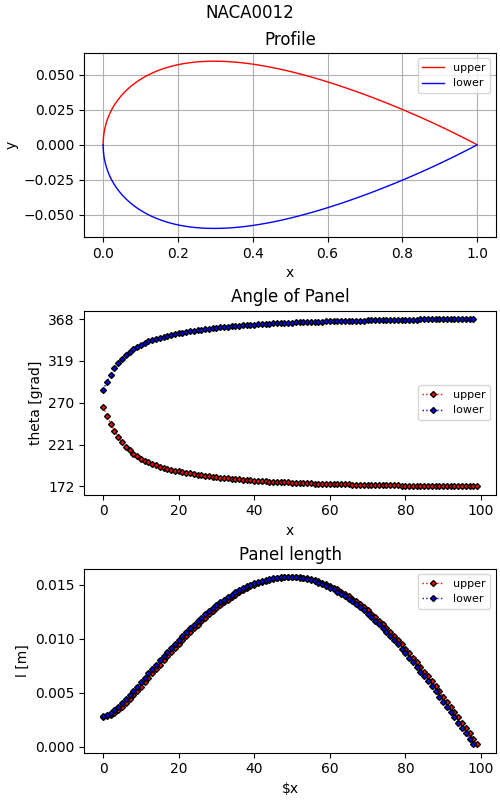
\includegraphics[scale=1]{figures/NACA0012.png} 
\caption{NACA-0012-Profil}
\label{fig:naca0012}
\end{center}
\end{figure}

\begin{table}
\label{tab:1}
\centering{
\begin{tabular}{cccc}
%\toprule
$X_i$ & $Y_i$         & $\theta_i$ & $l_i$ \\
%\midrule
0.8 & -0.35 & 67.5 & 0.77 \\
0.35 & -0.85 & 22.5 & 0.77 \\
-0.35 & -0.85 & 337.5 & 0.77 \\
-0.85 & -0.35 & 292.5 & 0.77 \\
-0.85 & 0.35 & 247.5 & 0.77 \\
-0.35 & 0.85 & 202.5 & 0.77 \\
0.35 & 0.85 & 157.5 & 0.77 \\
0.85 & 0.35 & 112.5 & 0.77

%\bottomrule
\end{tabular}
}
\end{table}

\begin{figure}[!h]
\begin{center}
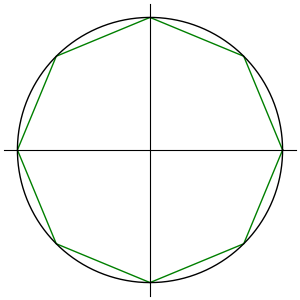
\includegraphics[scale=0.7]{figures/cylinderascircle.png} 
\caption{Achtseitiger Cylinder als Approximation eines Kreiszylinders sowie zugehörige Panelparameter}
\label{fig:cylinder8}
\end{center}
\end{figure}
\section{Untersuchungen am  Kreiszylinder}

Als nächstes wurden Untersuchung an Kreiszylindern vorgenommen, da bei diesen die Aufteilung in Panele relativ leicht zu implementieren ist. Zur Generierung eines Kreiszylinders mit $n$ gleich großen Seiten wurde die Funktion make\_cylinder(r, n) verwendet (siehe \nameref{appendix:c}).
\subsection{Achtseitiger Kreiszylinder}
\subsubsection{Berechnung der Systemmatrix}
Für den in \ref{fig:cylinder8} gezeigten Kreisylinder wurde die Systemmatrix zu folgenden Werten berechnet:
\begin{align*}
M_{i,j} = 
\begin{pmatrix}
0.5&0.056&0.064&0.065&0.065&0.065&0.064&0.056 \\
0.056&0.5&0.056&0.064&0.065&0.065&0.065&0.064\\
0.064&0.056&0.5&0.056&0.064&0.065&0.065&0.065\\
0.065&0.064&0.056&0.5&0.056&0.064&0.065&0.065\\
0.065&0.065&0.064&0.056&0.5&0.056&0.064&0.065\\
0.065&0.065&0.065&0.064&0.056&0.5&0.056&0.064\\
0.064&0.065&0.065&0.065&0.064&0.056&0.5&0.056\\
0.056&0.064&0.065&0.065&0.065&0.064&0.056&0.5
\end{pmatrix}
\end{align*}
\subsubsection{Lösung des wirbellosen Gleichungssystems}
\subsection{Untersuchungen an variierenden Kreiszylindern}
\subsubsection{Variation der Panelanzahl}
\subsubsection{Rotation des Zylinders}
\section{Untersuchungen an ausgewählten Profilen}
\subsection{NACA0012-Profil}
\subsection{Joukowsky 12\%-Profil}
\subsection{Fehlerabschätzung des Hess-Smith-Verfahrens}




\newpage